\section{Спектральный прибор и его основные характеристики - апаратная функция, линейная дисперсия, разрешающая способность и область дисперсии.}





\subsection{Дисперсионная область}




Область дисперсии - максимальная ширина спектрального интервала $\Delta \lambda$, при которой спектры соседних порядков еще не перекрываются. Если спектры начали накладываться друг на друга, данный прибор не позволяет исследовать данный интервал $\Delta \lambda$.

\begin{figure}[h!]
    \centering
    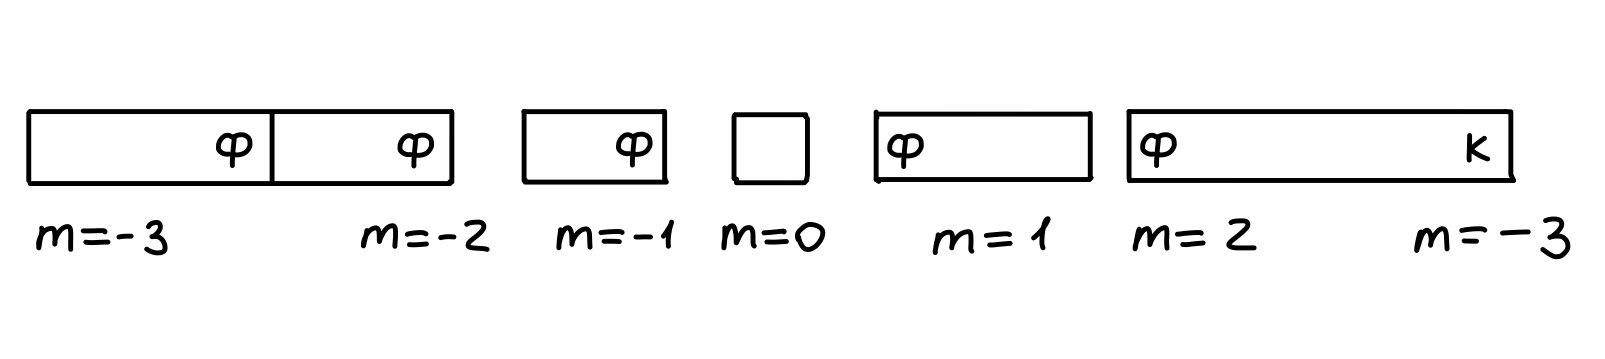
\includegraphics[scale=0.25]{34_1}
    \caption{Качественный вид дифракционной картины, получаемой дифракционной решеткой, на которую падает свет с конечной шириной спектра $\Delta\lambda$.}
    \label{fig:my_label}
\end{figure} 

Найдем условие, при котором начинается перекрытие. Возьмем спектральный диапазон $(\lambda,\lambda'), $  $\lambda' = \lambda  + \Delta \lambda.$  Главный максимум $m$-ого порядка для границы спектра $\lambda' $ имеет такое направление, что

\begin{equation*}
    d\sin\theta = m\lambda'.
\end{equation*}

Максимум $(m+1)$-ого порядка для границы спектра $\lambda$ должен распространяться под тем же углом, так что

\begin{equation*}
    d\sin\theta = (m+1)\lambda.
\end{equation*}

\begin{equation*}
    (m+1)\lambda = m\lambda' \Rightarrow m\Delta\lambda = \lambda \Rightarrow \Delta\lambda = \frac{\lambda}{m}.
\end{equation*}

Таким образом, спектры $m$-ого и $(m+1)$-ого порядка не перекрываются, если ширина спектрального диапазона достаточно мала:

\begin{equation*}
    \Delta \lambda \leq \frac{\lambda}{m}
\end{equation*}
\subsection{Угловая дисперсия}

Угловая дисперсия дифракционного прибора - это величина, определяемая равенством

\begin{equation*}
    D = \frac{d\theta}{d\lambda}
\end{equation*}

Она определяет угловое расстояние $d\theta$ между спектральными линиями, отстоящими по длине волны на $d\lambda$:
\begin{equation*}
   \Delta \theta \approx D \Delta \lambda
\end{equation*}

Например, для дифракционной решетки имеем
\begin{equation*}
    \sin \theta = m\frac{\lambda}{d}  \Rightarrow D = \frac{m}{d\cos\theta}
\end{equation*}

В частности, для малых углов дифракции

\begin{equation*}
    D = \frac{m}{d}
\end{equation*}

\subsection{Линейная дисперсия}

Линейная дисперсия - это расстояние между разрешаемыми линиями спектра на экране, на котором рассматривается дифракционная картина. 

\begin{figure}[h!]
    \centering
    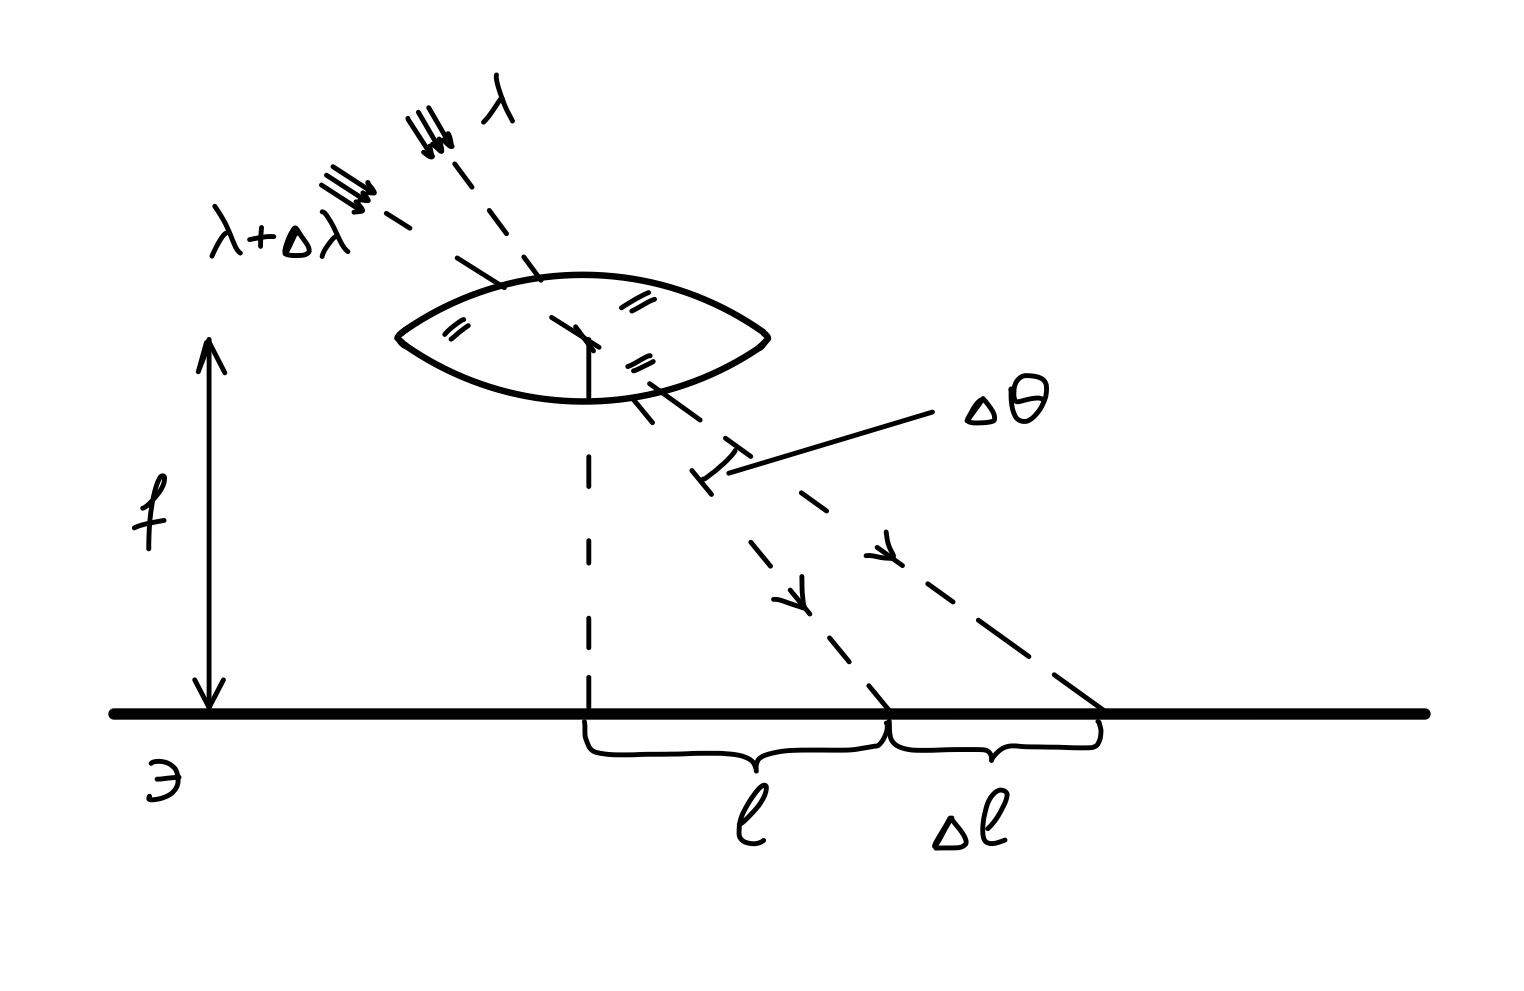
\includegraphics[scale=0.25]{34_2}
    \caption{Волны, отвечающие разным спектральным компонентам, отображаются с помощью линзы на экране в разные точки}
    \label{fig:my_label}
\end{figure} 


Отображая спектральные компоненты $\lambda$ и $\Delta \lambda$ в фокальной плоскости линзы, получаем линейное расстояние $\Delta l$ между ними на экране. Формально линейная дисперсия определяется равенством

\begin{equation*}
    D_{\text{лин}} = \frac{dl}{d\theta}
\end{equation*}

Поскольку $ dl = f\cdot d\theta$, то

\begin{equation*}
    D_{\text{лин}} = f \cdot D \approx \frac{fm}{d}
\end{equation*}

(Здесь использовано $D = \frac{m}{d}$ для дифракционной решетки)
\subsection{Разрешающая способность}

Разрешающая способность спектрального прибора - это величина, определяемая равенством

\begin{equation*}
    R = \frac{\lambda}{\Delta \lambda}, \text{где}
\end{equation*}

$\Delta \lambda$ - минимальная разность длин волн двух спектральных линий, которые воспринимаются раздельно.

\begin{figure}[h!]
    \centering
    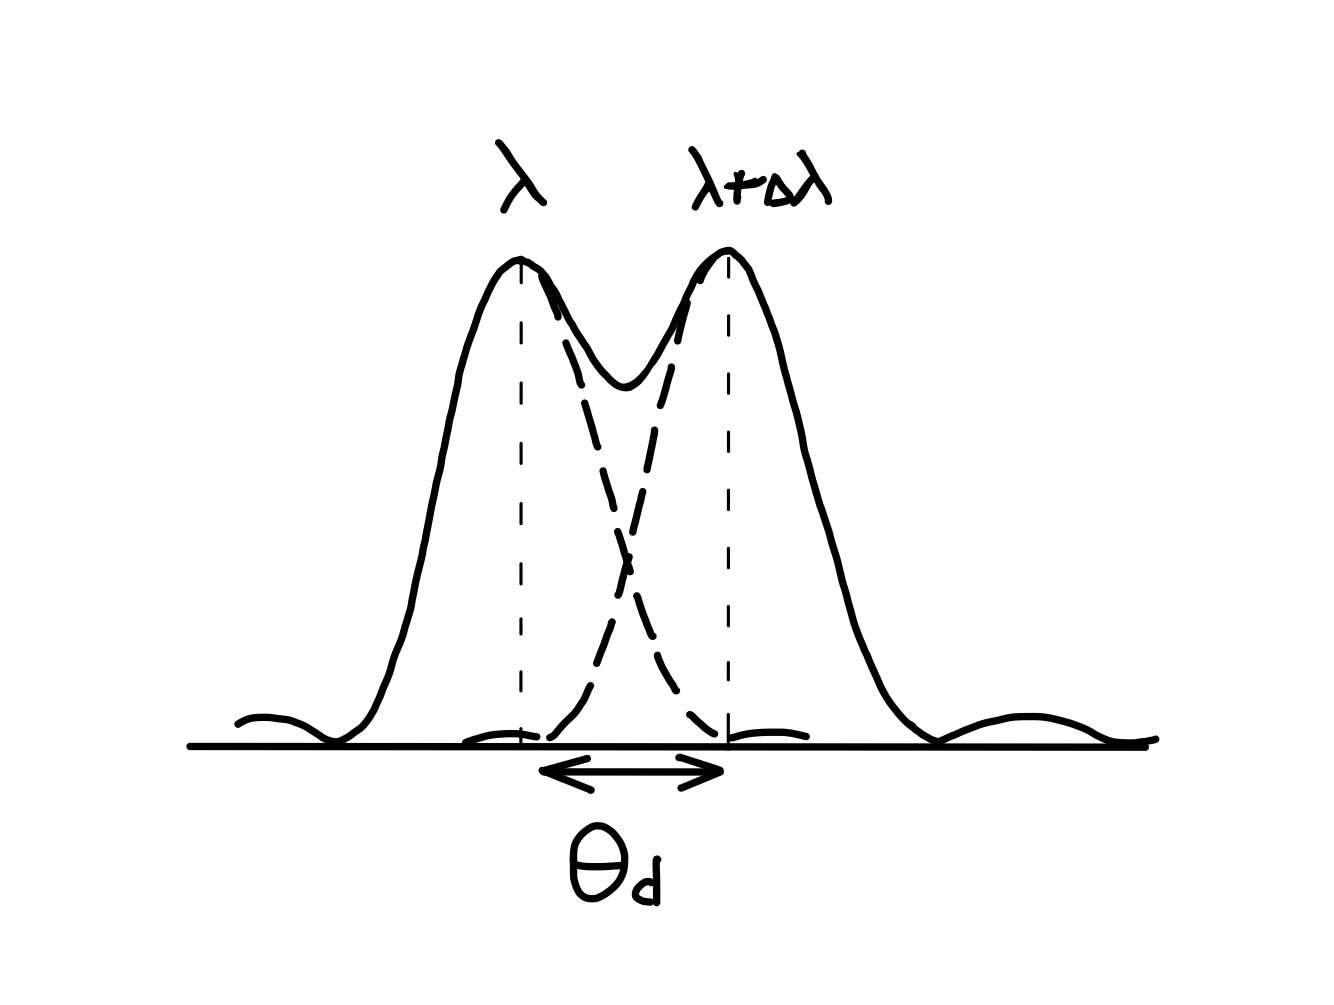
\includegraphics[scale=0.25]{34_3}
    \caption{Дифракционные пятна от двух компонент спектра, $\theta_d - $угловой радиус главного дифракционного максимума}
    \label{fig:my_label}
\end{figure} 


В качестве примера найдем разрешающую способность дифракционной решетки. Используем критерий Рэлея(см.рисунок). Пусть решетка имеет $N$ штрихов. Выберем главный максимум $m-$ого порядка для компоненты $\lambda$. Направление на первый дифракционный минимум даетмя равенством

\begin{equation*}
    d\sin \theta_d = \left(m + \frac{1}{N}\right) \lambda
\end{equation*}

Согласно критерию Рэлея компоненты считаются разрешенными, если это же направление соответствует главному дифракционнуму максимуму для второй компоненты $\lambda + \Delta \lambda$:

\begin{equation*}
    d\sin \theta_d = m(\lambda + \Delta\lambda)
\end{equation*}

\begin{equation*}
   \left(m + \frac{1}{N}\right) \lambda = m(\lambda + \Delta \lambda) \Rightarrow \Delta \lambda = \frac{\lambda}{mN}
\end{equation*}

Таким образом, получим разрешающую способность дифракционной решетки:

\begin{equation*}
   R = \frac{\lambda}{\Delta \lambda} = mN
\end{equation*}




